\documentclass[11pt,a4paper]{article}
\usepackage[latin1]{inputenc}
\usepackage[T1]{fontenc}
\usepackage{amsmath}
\usepackage{amsfonts}
\usepackage{amssymb}
\usepackage{graphicx}
\usepackage{here}
\usepackage{threeparttable, booktabs}
\usepackage{siunitx}
\usepackage{todonotes}
\usepackage{hyperref}
\usepackage{cleveref}
\usepackage[backend=biber]{biblatex}
	\addbibresource{refs.bib}

\author{Anders Brakestad, Luca Frediani, and Kathrin Helen Hopmann}
\title{Preliminary results: \\ BSSE-free association energies with MultiWavelets}
\begin{document}
	\maketitle
	\tableofcontents

\setcounter{secnumdepth}{2}

\section{Preface}
The aim of the project is to benchmark association reaction energies involving TM complexes with MRChem.
With a MW basis ``at'' the CBS limit, we automatically eliminate the BSSE, which is known to plague reaction energies.
We can therefore simplify the computational protocol by eliminating two birds with one stone: MW takes care of the BSIE problem related to GTO basis sets, and MWs also eliminate the need for carrying out annoying and complicated CP correction schemes.


\section{Computational details}
GTO calculations are run with ORCA version 4.2.1, and MW calculations are run with MRChem.

MW calculations performed with $\epsilon_{\text{rel}} = \num{1e-6}$

Several basis sets are currently tested: \verb|def2-svp|, \verb|def2-tzvp|, \verb|def2-qzvpp|, \verb|6-311g(d,p)|, and \verb|6-311+g(d,p)|.
Two functionals are currently being tested: \verb|bp86| and \verb|pbe0|.

Geometries are optimized with the \verb|def2-svp| basis set, with the following ORCA keyword line:

\begin{quote}
	\verb|! rks| \\
	\verb|! tightopt freq d3| \\
	\verb|! <functional> def2-svp grid5 finalgrid6| \\ 
	\verb|! ri(jcosx) autoaux gridx5|
\end{quote}

If imaginary frequencies are present, then retry optimization without RI(JCOSX) approximation.
This usually eliminates them.

Large-basis single-point calculations use the following keywords:

\begin{quote}
	\verb|! rks| \\
	\verb|! <functional> <basis_set> grid5 finalgrid6 d3 tightscf|
\end{quote}

The BSSE is computed by Boys' and Bernardi's counterpoise correction, with the BSSE given by

\begin{equation} \label{eq: bsse}
\text{BSSE} = \Big(\Delta E^{\text{A}}_{\text{(A)}} - \Delta E^{\text{A}}_{\text{(AB)}} \Big) + \Big( \Delta E^{\text{B}}_{\text{(B)}} - \Delta E^{\text{B}}_{\text{(AB)}}\Big )			
\end{equation}

where the superscript indicates the molecular geometry and the subscript indicates the basis set.
This equation is easily derived from the following argument.
If the uncorrected and CP-corrected reaction energies are

\begin{align} \label{eq: rxn uncorrected}
\Delta E &= E^{\text{AB}}_{\text{(AB)}} - E^{\text{A}}_{\text{(A)}} - E^{\text{B}}_{\text{(B)}} \\ \label{eq: rxn corrected}
\Delta E^{\text{CP}} &= E^{\text{AB}}_{\text{(AB)}} - E^{\text{A}}_{\text{(AB)}} - E^{\text{B}}_{\text{(AB)}}
\end{align}

then the error (\cref{eq: bsse}) is the difference between them.
The corrected reaction energy then becomes

\begin{equation} \label{eq: }
\Delta E^{\text{CP}} = \Delta E + \text{BSSE}
\end{equation}

\section{Reactions studied}
	\subsection{New set}
	Figure showing all association reactions are not ready yet.
	
	
	\subsection{Old set}
	The reaction numbers refer to the same indeces used in \textcite{dohm2018}.
	Note that reaction 12b is the same as reaction 12 but using trans-stilbene instead of ethene.

\section{Overview of BSSE for the new reactions}
\Cref{fig: bsse overview} presents the BSSE for all basis sets and all reactions. 
Systems with larger BSSEs may be of special interest in the benchmark, since the impact of
the MRChem calculations may be larger.
The figure shows that the Ni complexes exhibit larger BSSEs than the Cr complexes with the same ligands.
A possible rationalization: Ni has more electrons than Cr, and thus more basis functions.
Further, the tetrahedral geometry may lead to a larger electron density close to the metal, and thus in the overlapping region with the associating ligand, and therefore more basis functions, than the for the octahedral geometry.

\begin{figure}[H]
	\centering
	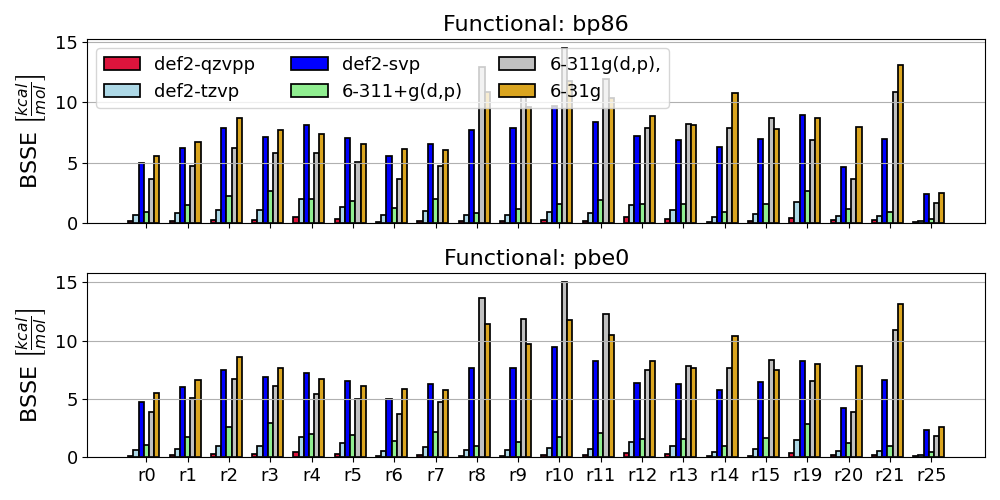
\includegraphics[width = \textwidth]{../figs/bsse.png}
	\caption{BSSEs for all BP86 (top) and PBE0 (bottom). Reactions 8--15 (Ni complexes) seem to have larger BSSEs than reactions 0--7 (Cr complexes).}
	\label{fig: bsse overview}
\end{figure}

\section{OLD: Reaction energies, GTOs vs MWs}
In order to compare reaction energies computed from GTOs and MWs, we use the relative error metric:

\begin{equation} \label{eq: relative error}
\text{RE} = \frac{\Delta E^{\small\text{GTO}} - \Delta E^{\small\text{MW}}}{\Delta E^{\small\text{MW}}} \times 100\%
\end{equation}

There is no point in using ZPE or D3 corrections for the reaction energies, because the ZPE and D3 corrections are identical for the GTO and MW reaction energies.
When computing the difference, the corrections cancel exactly:

\begin{align} \label{eq: }
 \Delta H^{\small\text{GTO}} &= \Delta E^{\small\text{GTO}} + \Delta \text{D3} + \Delta \text{ZPE} \\
  \Delta H^{\small\text{MW}} &= \Delta E^{\small\text{MW}} + \Delta \text{D3} + \Delta \text{ZPE} \\
  \Delta H^{\small\text{GTO}} - \Delta H^{\small\text{MW}} &= \Delta E^{\small\text{GTO}} - \Delta E^{\small\text{MW}}
\end{align}

The correct expression for the RE is therefore to use the electronic reaction energies.

	\subsection{Non-CP corrected}
	Reaction energies from GTO calculations \textbf{without} CP correction compared to MW reaction energies.
	\begin{figure}[H]
		\centering
		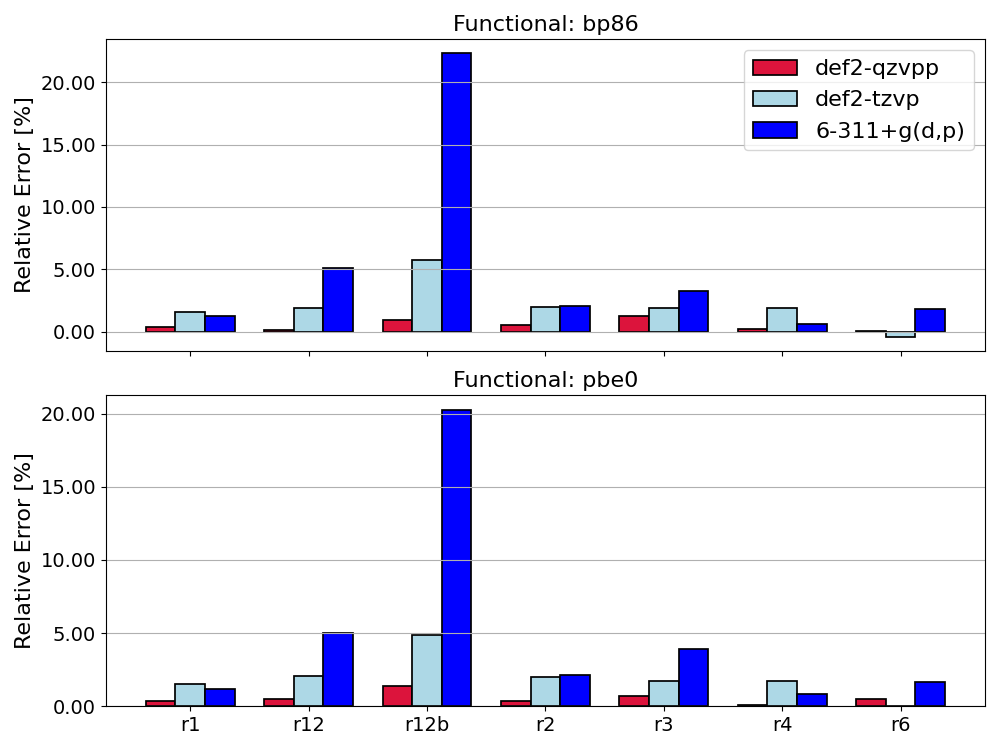
\includegraphics[width = \textwidth]{../figs/old_gto_vs_mw_noncp.png}
		\caption{Relative errors comparing GTO reaction energies (without CP) with MW reaction energies.}
		\label{fig: }
	\end{figure}

	\subsection{CP-corrected}
	Reaction energies from GTO calculations \textbf{with} CP correction compared to MW reaction energies.
	\begin{figure}[H]
		\centering
		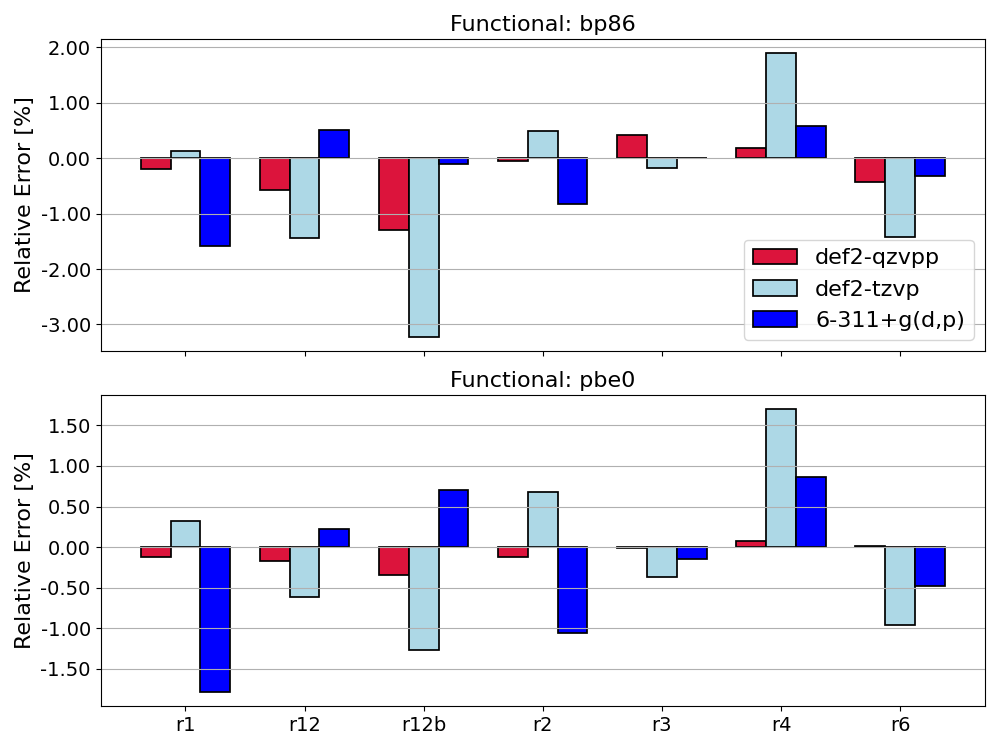
\includegraphics[width = \textwidth]{../figs/old_gto_vs_mw_cp.png}
		\caption{Relative errors comparing CP-corrected GTO reaction energies with MW reaction energies.}
		\label{fig: }
	\end{figure}

	\subsection{Computed reaction energies}
	Here is presented the D3 and CP reaction energies for various GTO basis sets and high-precision MWs. The reference value\parencite{dohm2018} is also showed in the tables.
	
	\begin{table}[H]
		\centering
		\label{tab: rxn energies old bp86}
		\caption{CP-corrected reaction energies (\si{kcal/mol}) with BP86 for the old set of reactions. D3 corrections have been applied to GTO and MW reaction energies. Reaction energies without CP-correction are given in parenthesis. No ZPE corrections applied.}
		\begin{tabular}{l l l l l l }
			\toprule
			Reaction & def2-tzvp       & 6-311+g(d,p)    & def2-qzvpp      & MW6    & Reference \parencite{dohm2018} \\ \midrule
			r1       & -47.38 (-46.77) & -47.23 (-46.05) & -46.86 (-46.63) & -46.71 & -43.1                          \\
			r12      & -29.36 (-28.60) & -30.09 (-29.05) & -28.95 (-28.80) & -28.93 & -29.8                          \\
			r12b     & -32.13 (-31.09) & -34.07 (-31.45) & -31.57 (-31.31) & -31.46 &                                \\
			r2       & -50.43 (-49.78) & -50.48 (-49.18) & -49.80 (-49.53) & -49.56 & -46.6                          \\
			r3       & -31.50 (-30.94) & -31.90 (-30.99) & -31.33 (-31.10) & -30.99 & -27.6                          \\
			r4       & -75.75 (---)    & -74.83 (---)    & -74.56 (---)    & -74.42 & -62.5                          \\
			r6       & -18.18 (-18.00) & -18.57 (-18.20) & -18.25 (-18.18) & -18.25 & -23.2                          \\ \bottomrule
		\end{tabular}
	\end{table}

\begin{table}[H]
	\centering
	\label{tab: rxn energies old pbe0}
	\caption{CP-corrected reaction energies (\si{kcal/mol}) with PBE0 for the old set of reactions. D3 corrections have been applied to GTO and MW reaction energies. Reaction energies without CP-correction are given in parenthesis. No ZPE corrections applied.}
	\begin{tabular}{l l l l l l}
		\toprule
		Reaction & def2-tzvp       & 6-311+g(d,p)    & def2-qzvpp      & MW6    & Reference \parencite{dohm2018} \\ 
		\midrule
		r1       & -45.30 (-44.80) & -45.16 (-43.92) & -44.81 (-44.62) & -44.67 & -43.1                          \\
		r12      & -29.53 (-28.84) & -30.28 (-29.05) & -29.12 (-28.95) & -29.00 & -29.8                          \\
		r12b     & -27.40 (-26.45) & -29.78 (-26.76) & -26.86 (-26.60) & -26.65 &                                \\
		r2       & -48.49 (-47.90) & -48.56 (-47.11) & -47.74 (-47.54) & -47.59 & -46.6                          \\
		r3       & -26.80 (-26.28) & -27.33 (-26.33) & -26.54 (-26.37) & -26.37 & -27.6                          \\
		r4       & -72.56 (---)    & -71.98 (---)    & -71.44 (---)    & -71.39 & -62.5                          \\
		r6       & -20.41 (-20.21) & -20.74 (-20.31) & -20.50 (-20.40) & -20.40 & -23.2                          \\ 
		\bottomrule
	\end{tabular}
\end{table}
	

\printbibliography

\end{document}
